\documentclass[a4paper,12pt]{report}
\usepackage[top=1in, bottom=1in, left=1in, right=1in]{geometry} % Custom margins
\usepackage[dutch]{babel}
\usepackage[T1]{fontenc} % Special chars
\usepackage{graphicx} % \includegraphics
\graphicspath{{./img/}}
\usepackage[hidelinks]{hyperref} % \url
\usepackage{pdfpages} % \includepdf
\usepackage{tocbibind} % Custom toc entries
\usepackage{listings} % Code snippets
\lstdefinestyle{code}{
  basicstyle=\ttfamily\footnotesize,
  breakatwhitespace=false,         
  breaklines=true,                 
  captionpos=b,                    
  keepspaces=true,                 
  numbers=left,                    
  numbersep=5pt,                  
  showspaces=false,                
  showstringspaces=false,
  showtabs=false,                  
  tabsize=2
}
\lstset{style=code}
\usepackage{blindtext} % Lorem ipsum
\usepackage[backend=biber,style=apa]{biblatex} % References
\addbibresource{references.bib}

\title{Implementatie van een NIDS binnen een ISP omgeving}
\author{Jonas Meeuws}

\begin{document}

% Bedrukte kaft (=titelblad)

\includepdf[pages=-]{./include/titelblad.pdf}

% Schutblad
\newpage
\thispagestyle{empty}
\mbox{}

% Titelblad

\includepdf[pages=-]{./include/titelblad.pdf}

% Mededeling
\chapter*{Mededeling}
\addcontentsline{toc}{chapter}{Mededeling}
Deze eindverhandeling was een examen.
De tijdens de verdediging geformuleerde opmerkingen werden niet opgenomen.

% Woord vooraf (niet verplicht)
\chapter*{Woord vooraf}
\addcontentsline{toc}{chapter}{Woord vooraf}
% Hier heb je de mogelijkheid om je waardering uit te drukken en dank te betuigen. Je neemt in
% het woord vooraf geen gegevens op die essentieel verband houden met het behandelde
% onderwerp (methode, doelstelling, enz.).
\blindtext

% Samenvatting of abstract
\chapter*{Samenvatting}
\addcontentsline{toc}{chapter}{Samenvatting}
\blindtext

% Inhoudsopgave
\tableofcontents
\newpage

% Lijst van figuren (niet verplicht)
\listoffigures

% Inleiding
\chapter*{Inleiding}
\addcontentsline{toc}{chapter}{Inleiding}
\blindtext

% Inhoud
\chapter{Intrusion detection}
Intrusion detection is het monitoren van systemen op verdachte activiteit.
Dit omvat pogingen tot hacken, verspreiding van virussen of malware, aanwezigheid van rogue devices\dots

Intrusion detection gebeurt typisch volledig passief.
De logs die een IDS (Intrusion detection system) produceert kunnen worden verstuurd naar een administrator als een alert.
In grotere systemen worden deze logs centraal verzameld om deze anomalieën effectief te kunnen analyseren.
\autocite{wikipedia:ids}

Intrusion detection systemen worden opgedeeld in 2 soorten: network (NIDS) en host (HIDS) intrusion detection.

\section{NIDS}
Een network intrusion detection systeem (NIDS) monitort een netwerkverbinding.

De 2 grote NIDS software projecten zijn Snort en Suricata.
Voor een groot deel werken de 2 systemen identiek voor een eindgebruiker.
Zo is de NIDS rule syntax van Snort en Suricata bijna gelijk.
Het verschil ligt in specifieke features (zie \url{https://suricata.readthedocs.io/en/suricata-5.0.3/rules/differences-from-snort.html} voor een gedetailleerde lijst van verschillen).

\subsection{Regels}
Een NIDS monitort gecapteerd netwerkverkeer aan de hand van een lijst van regels.
Deze regels volgen een bepaalde syntax.

Een voorbeeld van een nids rule is als volgt (figuur \ref{fig:nids-rule}).

\begin{figure}[h]
  \begin{lstlisting}
alert tcp $EXTERNAL_NET any -> $INTERNAL_NET 3306 (msg:"Inbound SQL connection"; sid:1000000;)
  \end{lstlisting}
  \caption{Een nids rule.}
  \label{fig:nids-rule}
\end{figure}

Deze rule zorgt ervoor dat er een alert wordt gegenereerd wanneer de NIDS engine een tcp verbinding ziet van het extern netwerk naar het intern netwerk op poort 3306.
Het extern netwerk is meestal het internet of een WAN, het intern netwerk is meestal een LAN.
Volgens het tcp client-server model is de client een externe host en de server een interne host.

Poort 3306 is gereserveerd voor MySQL database verbindingen \autocite{iana:ports}.
Deze verbindingen kunnen perfect normaal zijn als de client een vertrouwde host is.
In dit geval is de client echter een externe host die acties probeert uit te voeren op een interne MySQL database.
Dit is verdachte activiteit, vandaar het type alert.

% Voorbeeld downloaded rules

\subsection{Variabelen}
Om regels zo effectief mogelijk te maken, worden er variabelen geïntroduceerd.

De 2 meest gebruikte variabelen zijn het \lstinline|INTERNAL_NET| en het \lstinline|EXTERNAL_NET|.
Bijna alle regels gebruiken minstens 1 van deze variabelen, daarom is het van groot belang om deze in te stellen.
Als een variabele niet ingesteld is, worden regels die deze variabele gebruiken genegeerd.

Variabelen kunnen ook de waarde \lstinline|any| aannemen.
Dit kan zorgen voor veel false alerts, maar is wel nuttig in gesloten netwerken waar incidenten zich enkel intern afspelen.

% Subscription models
% strategisch plaatsen
\subsection{Port mirror}
% Limitatie linksnelheid (of andere term)
% Schets hoe het netwerk eruit ziet tov de mirror op laag 2 en op laag 3 voor of na de NAT
Een NIDS engine zoals Snort of Suricata wordt normaal gebruikt om te capteren op 1 netwerkinterface.
Deze interface ontvangt typisch een kopie van een punt in het netwerk.
Dit noemt men een port mirror.

Een voorbeeld van een technologie die port mirroring toelaat is SPAN.
Deze is aanwezig in bijvoorbeeld een switch en kopieert alle pakketten van een source poort naar een destination poort.
Daarnaast kan RSPAN gebruikt worden om gecapteerde pakketten over een laag 2 netwerk te transporteren.
Ten slotte kan ERSPAN op de zelfde manier gebruikt worden om een port mirror te transporteren over een laag 3 netwerk.
\autocite{cisco:span}

Het geheel van een NIDS engine die al het netwerkverkeer op 1 punt in een netwerk capteert, noemt men een sensor.
Eén of meerdere sensoren kunnen in een netwerk geplaatst worden op strategische punten.
Dit zijn vaak plaatsen waar een vertrouwd netwerk wordt verbonden met een extern netwerk.

De meest interresante plaats om een sensor te plaatsen in een bedrijfsnetwerk is meestal de plaats waar NAT toegepast wordt.
Dit is omdat alle communicatie met externe netwerken doorheen dit punt passeert.
Als zo'n sensor aan de buitenkant van de NAT staat, zijn de interne ip-adressen niet zichtbaar.
We zien enkel ip-communicatie tussen de NAT-pool en externe netwerken, zo gaat er veel informatie verloren.
Daarom gaat de voorkeur naar het plaatsen van de sensor aan de binnenzijde van de NAT.

Waar men ook voor moet uitkijken bij het plaatsen van een sensor is of de hardware de bitsnelheid wel aankan.
Als de link tussen de port mirror en de sensor een lager maximum bits/s heeft dan bitsnelheid van de combinatie van de beide richtingen van de te capteren poort, kan er packet loss optreden.
NIDS engines kunnen hiermee wel overweg, maar het zorgt natuurlijk voor verlies van informatie.

\section{HIDS}
% Omschrijving principe: agents op clients loggen naar een master server
% Niet uitgebreid
% Zelf nooit gebruikt, nog opzoeken

\chapter{Security Onion}
\section{Wat is Security Onion?}
De officiële site beschrijft Security Onion als:
``Security Onion is a free and open source Linux distribution for intrusion detection, enterprise security monitoring, and log management.
It includes Elasticsearch, Logstash, Kibana, Snort, Suricata, Zeek, Wazuh, Sguil, Squert, CyberChef, NetworkMiner, and many other security tools.''
\autocite{so:docs}

\section{Geschiedenis}
In 2008 begon Doug Burks met het ontwikkelen van Security Onion.
Een eerste versie van het project werd gepubliceerd in 2009.
Omdat de Linux distributie meer populariteit kreeg, werd het in 2012 volledig herschreven met het doel om performantie en schaalbaarheid te verbeteren.
In 2014 werd Security Onion Solutions LLC opgericht om professionele ondersteuning aan te bieden aan bedrijven.
Met jaarlijkse conferenties bleef het project groeien.
\autocite{so:sos}
In 2018 begon de ontwikkeling van een nieuw project, Security Onion Hybrid Hunter.
Hybrid Hunter is nog steeds in experimentele staat, en het wordt afgeraden dit systeem te gebruiken in een productieomgeving.

\section{Features}
Security Onion heeft veel te bieden om een goed inzicht te krijgen grote hoeveelheden netwerkverkeer waar standalone tools als Suricata of Wireshark te onoverzichtelijk worden.

\subsection{NIDS}
Als een deels afgesloten systeem is er NIDS.
Dit bestaat uit een NIDS engine, ofwel Snort ofwel Suricata, die binnenkomende pakketten vergelijkt met een lijst van rules en al dan niet een alert van bepaalde prioriteit genereert.
Die alerts worden verzonden naar beide Logstash en Sguild.

In Logstash worden de alerts behandeld als logs.
Deze logs zijn dan zichtbaar in Elasticsearch en Kibana.

Sguild is een database voor IDS alerts.
De frontend tools Sguil en Squert voeren queries uit op deze database om de alerts aan de analyst te presenteren.

De HIDS info van OSSEC is ook zichtbaar in beide Elasticsearch en Sguild, maar dit is standaard beperkt tot de OSSEC daemons die op de Security Onion servers zelf opereren.

Mijn voorkeur van NIDS engine gaat naar Suricata, vooral omdat het moderner is.
Suricata heeft afgewerkte ondersteuning voor multithreading en naar mijn mening betere documentatie.

Bij het analyseren van alerts heb ik vooral Squert gebruikt.
Opnieuw is dit een veel gebruiksvriendelijkere en moderne tool dan Sguil.
Sguil heeft wel bepaalde mogelijkheden die ontbreken bij Squert zoals het manueel uitvoeren van SQL queries op de Sguild database.

\subsection{Zeek}
Security Onion definieert een sensor als een verzameling van services die actief zijn op 1 netwerkinterface.
Alle configuratie voor 1 zo'n sensor bevindt zich in een map \lstinline|/etc/nsm/[hostname]-[interface]|.
Naast Suricata of Snort (de NIDS engine) is er nog een andere service die de gecapteerde pakketten analyseert.
Deze service is Zeek.

Zeek (vroeger Bro) is een open-source analyser voor netwerkverkeer.
Van de officiële documentatie:
``Zeek is a passive open-source network traffic analyzer.
It is primarily a security monitor that inspects all traffic on a link in depth for signs of suspicious activity.
More generally, however, Zeek supports a wide range of traffic analysis tasks even outside of the security domain, including performance measurements and helping with trouble-shooting.''
\autocite{zeek:docs}

Zeek heeft de mogelijkheid om gedetailleerde logs te genereren van veel verschillende soorten netwerkverkeer.
Bij tcp verbindingen wordt er bijvoorbeeld bijgehouden wat de source en destination poort was, hoeveel data er uitgewisseld is geweest en hoe de verbinding beëindigd werd.
Udp en icmp pakketten worden gelijkaardig behandeld.
Bij applicatielaag protocollen worden er veel details gehaald uit de plain-text protocollen zoals HTTP, FTP, DNS, MySQL\dots
Ook geëncrypteerde protocollen die SSL gebruiken worden geanalyseerd op \emph{self-signed} en verlopen certificaten.

Enkele velden komen in bijna elke log voor, zoals het source en destination ip-adres.
Hierdoor is het mogelijk om snel correlaties te vinden in verschillende logs met een tool als Kibana.

Deze logs zijn beschikbaar in json-formaat in \lstinline|/nsm/bro/logs|.
De logs worden geconsumeerd door syslog-ng.
Daarna komen ze terrecht in de ELK stack, waar er meer informatie wordt toegevoegd en ze uiteindelijk zichtbaar zijn in Kibana.
\autocite{so:docs}

\subsection{ELK stack}
ELK staat voor Elasticsearch, Logstash, and Kibana.
De ELK stack is een open-source systeem voor het beheren en visualiseren van data (logs) van meerdere bronnen.

Logstash neemt data binnen van verschillende bronnen zoals NIDS, HIDS en Zeek, verrijkt deze bronnen met bijvoorbeeld links naar de volledige pcap files en slaat deze logs op in elasticsearch.
Elasticsearch heeft een uitgebreide api om allerlei soorten zoekopdrachten uit te voeren op deze logs.
Een analyst kan dan de browser gebaseerde tool Kibana gebruiken om de logs in elasticsearch te visualiseren.
\autocite{elastic:what-is-elk}

Security Onion voorziet uitgebreide logs in elasticsearch die alle informatie van NIDS, HIDS en Zeek omvatten.
In Kibana zijn er een 40-tal dashboards aanwezig met in totaal zo'n 400 visualisaties.
Dit is zeker de meest handige tool voor een analyst, Kibana stond aan de kern van elke analyse die ik uitvoerde.

% elastalert

\section{Deployment scenario's}
Security Onion kan op verschillende manieren geïnstalleerd worden.
Dankzij de architectuur van het gehele systeem kunnen bepaalde taken weggenomen worden van de ene server, zodat een andere server met meer geschikte hardware deze taken kan behandelen.
Dit proces noemt men offloading.

\subsection{Evaluation Mode}
Een eerste mogelijkheid is \emph{Evaluation Mode}.
Deze is ideaal om de distributie te verkennen zonder het volledig te installeren in een productieomgeving, maar ook om pcap bestanden offline te analyseren met de kracht van het volledige systeem.

\subsection{Standalone Production Mode}
Een tweede mogelijkheid die beter geschikt is voor permanente opstellingen is de \emph{Standalone Production Mode}.
Hierbij werkt het volledige systeem vanaf 1 server: zowel de sensor, log management, opslag als de web interface vinden plaats op dezelfde \emph{Master node}.
Zie figuur \ref{fig:so-architecture-standalone} voor een schema.
\begin{figure}[h]
  \centering
  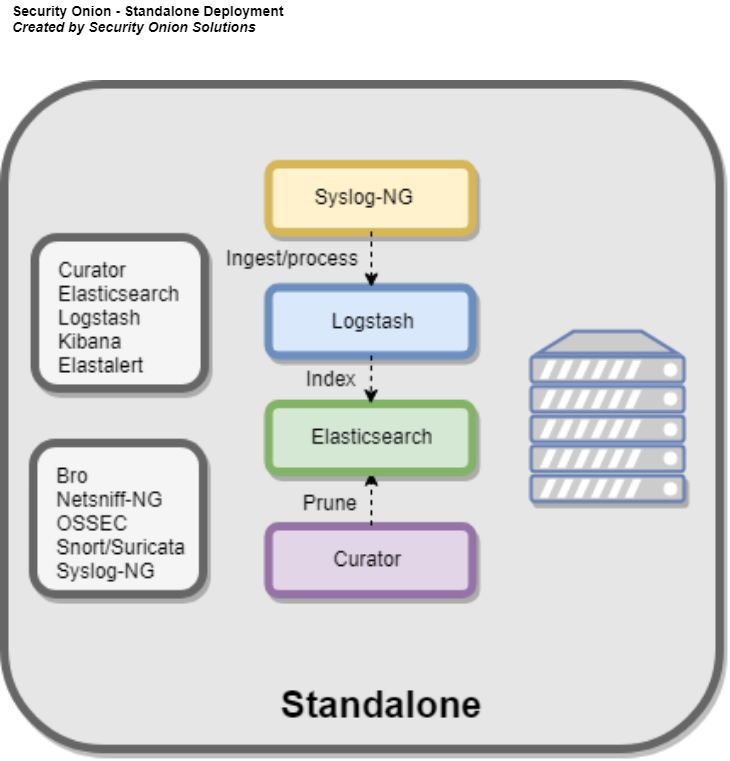
\includegraphics[width=0.5\textwidth]{so-architecture-production-standalone}
  \caption{Standalone Production deployment \autocite{so:docs}}
  \label{fig:so-architecture-standalone}
\end{figure}

\subsection{Distributed Production Mode}
Het laatste mogelijke scenario bestaat uit meerdere nodes met elk een unieke rol.
Zie figuur \ref{fig:so-architecture-distributed} voor een schema.

Elke node heeft standaard een OSSEC daemon actief.
Deze dient om aan Host-based intrusion detection te doen op het Security Onion systeem zelf.

\subsubsection{Forward node}
Een \emph{Forward node} bezit alle functies van een sensor.
Op elke forward node worden er 1 of meerdere port mirrors geïnstalleerd.
De gecapteerde pakketten worden door enkele services verwerkt: Netsniff-NG voor full packet capture, Zeek protocol decoding en Snort of Suricata als NIDS engine.
Alle logs die Zeek en Suricata of Snort genereren worden meteen doorgestuurd naar de Logstash instantie op de master server.
De full packet capture van netsniff-ng, blijft echter op de forward node aanwezig.
Deze pcap files kunnen opgehaald worden wanneer ze nodig zijn en worden automatisch verwijderd wanneer er te weinig vrije plaats is op de disk.

Door meerdere forward nodes strategisch te plaatsen in een netwerk, kan er veel beter inzicht verkregen worden in het netwerk.

\subsubsection{Master node}
De master node is standaard verantwoordelijk voor alle andere taken die geen raw pcap data verwerken.
Log management services zoals Elasticsearch, Logstash en Sguild zijn hier actief en frontend applicaties voor de analyst zoals Kibana en Squert worden hier gehost.

\subsubsection{Storage node}
Storage nodes kunnen gebruikt worden om de opslagcapaciteit uit te breiden en het verwerken van logs te verlichten voor de master node.

\subsubsection{Heavy node}
Heavy nodes zijn een combinatie van storage nodes en forward nodes.
Deze worden afgeraden om te gebruiken, maar kunnen wel gebruikt worden wanneer forward en storage nodes niet gesplitst kunnen worden omwille van bijvoorbeeld beperkte hardware.

\autocite{so:docs}

\begin{figure}[h]
  \centering
  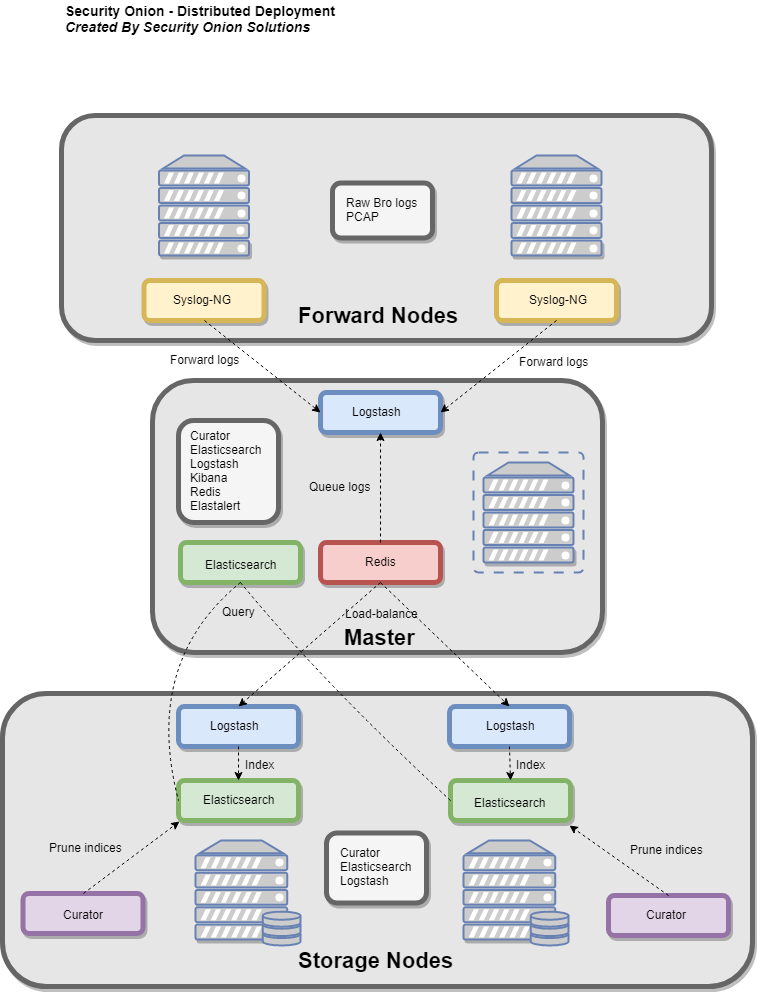
\includegraphics[width=0.6\textwidth]{so-architecture-production-distributed}
  \caption{Distributed Production deployment \autocite{so:docs}}
  \label{fig:so-architecture-distributed}
\end{figure}

\chapter{Installatie}
\section{Simulaties met GNS3}
% GNS3 uitleggen
\subsection{Appliances}
% Systeem van appliances
% Custom appliance voor SO + screenshot en/of code
\subsection{Simulatie bedrijfsnetwerk}
% Simulatie tonen van forward + master aan de NAT van een typisch bedrijfsnetwerk
\subsection{Cloud}
% GNS3 cloud component die toelaat fysieke interfaces te verbinden
% Echte data aan de simulatieomgeving koppelen
% Geen simulatie meer, maar een proof of concept

\section{Server}
\label{sec:server}
Tijdens mijn stage bij Fluvius kreeg ik een rack-mounted server ter beschikking.
Het was de bedoeling om deze in een serverruimte te plaatsen waar er 2 utp kabels voorzien werden.
Deze 2 kabels werden aangesloten op 2 netwerkinterfaces van de server.
De eerste diende als management interface, op deze interface moest een statisch publiek IPv4 adres geconfigureerd worden.
De tweede interface kreeg een port mirror van een netwerk binnen Fluvius.

Deze server configureerde ik eerst op een andere locatie, waar ik fysieke toegang had tot de server.
Eerst zorgde ik dat het host OS geïnstalleerd was, de netwerkconfiguratie aangepast was en toegang op afstand beschikbaar was via ssh.
Dan verwijderde ik de tijdelijke internetverbinding, stelde ik het statisch publiek ip adres in en testte of dit werkte.
Ten slotte werd deze server geïnstalleerd in de serverruimte, waarna ik fysieke toegang verloor.
De server moest altijd operationeel blijven en de toegang op afstand mocht nooit verloren gaan.

\chapter{Ontwikkelen van een aangepast systeem}
% Proberen schema hier te verwerken
\section{Motivatie}
Na het bekijken van de opnames van enkele presentaties van de Security Onion Conference 2019, bemerkte ik dat er veel mensen proberen externe tools te integreren met Security Onion.
\autocite{so:conference-2019}
Vaak is het doel om in de eerste plaats meer informatie te verzamelen aan de hand van bijvoorbeeld het raadplegen van externe bronnen.
Daarna moet die informatie centraal beschikbaar gesteld worden in een tool als Kibana.

\section{Gebruikte technologie\"en}
\subsection{Debian}
Heel dit systeem is aanwezig op de server eerder besproken in sectie \ref{sec:server}.
In de eerste plaats was er een OS nodig om dit systeem op uit te voeren.

In de keuze van besturingssysteem waren 2 zaken belangrijk.
Het OS moest zeer stabiel zijn, het mocht nooit crashen tijdens het ontwikkelen of uitvoeren van dit systeem.
Daarnaast moest ik altijd de toegang op afstand bewaren.
Omwille van deze redenen koos ik de huidige \emph{stable} branch van Debain: Debian Buster.

\subsection{Docker}
% Docker presenteren als tool om linux containers of namespaces (een kernel feature) te beheren
% Docker kan een stuk meer zoals met windows containers, maar dit is alles wat we gebruiken
Docker is een verzameling van tools voor het beheren van software containers.
Deze containers zijn applicaties gebundeld met al hun dependencies en configuratie.
Docker is beschikbaar voor enkele verschillende omgevingen, maar voor dit systeem wordt enkel de Linux versie gebruikt.

Docker gebruikt enkele Linux kernel features, vooral Linux namespaces die toelaten om zaken zoals bestandssystemen en de netwerk stack te isoleren.
Dit zorgt ervoor dat Docker containers een volledig andere installatie van Linux kunnen bevatten, het enige wat hetzelfde blijft is de achterliggende Linux kernel.

Dit isolatie systeem zorgt ervoor dat er enkele handige features aanwezig zijn in Docker.
Zo kunnen bestanden, mappen en zelfs Unix sockets gelinkt worden tussen host en container.
Ook kunnen tcp of udp poorten geforward worden naar interfaces van de host en kunnen er ip netwerken gemaakt worden tussen verschillende containers en de host.

Docker kan door softwareontwikkelaars gebruikt worden om hun applicaties samen met alle nodige libraries en andere dependencies, als 1 pakket te publiceren.
Deze applicaties kunnen dan gedownload worden als een Docker image.
Docker kan ook gebruikt worden bij het ontwikkelen van systemen die bestaan uit meerdere applicaties.
Een typisch voorbeeld hiervan is een webserver en een database.
De http poort van de webserver container wordt dan geforward naar de host en de database container is bereikbaar via een intern netwerk waar beide containers mee verbonden zijn.

% Docker logo

% Evt Dockerfiles tonen

\subsubsection{Dockerfiles}

\autocite{docker:containers}

\subsubsection{Docker compose}
% Github repo presenteren
% Indien het overzichtelijk gebruikt wordt, tool om het volledige systeem mee te ontwerpen
% Compose files tonen

\subsection{Libvirt}
% Open source hypervisor
% Werkt samen met qemu en KVM
% Uitleggen wat een hypervisor is en bekende alternatieven zoals hyper-v (windows) en virtualbox aanhalen

\section{Intern netwerk}
% SO en so-poc zitten in een apart /24 subnet
% 1 wordt beheerd door docker, het andere door libvirt
Vanuit het perspectief van het host besturingssysteem Debian, zijn er 4 interfaces actief.
Deze bestaan uit de management poort, de capture poort, een Libvirt virtueel netwerk en een Docker intern netwerk.

\subsubsection{Management poort}
De management poort is rechtsreeks verbonden met het internet en heeft een statisch publiek ip.
Enkel de poorten voor ssh, http en https zijn actief.
Ssh is beveiligd met een whitelist van geauthoriseerde publieke sleutels, in deze whitelist staan enkel sleutels van mijn persoonlijke apparaten.
De http poort geeft steeds een redirect naar de https poort, tenzij bij het ophalen van nieuwe https certificaten bij \emph{Let's Encrypt}.
Op de https poort zijn alle web services beschikbaar, maar er is steeds een gebruikersnaam en wachtwoord nodig in de vorm van \emph{HTTP basic access authentication} om toegang te krijgen tot deze services.

\subsubsection{Capture poort}
Op de capture poort komt er een port mirror toe.
Toegang tot deze capture poort wordt verspreid naar de verschillende services die deze data nodig hebben.
In Libvirt gebeurt dit via de interface passthrough feature.
In Docker kunnen bepaalde containers toegang krijgen tot het `host net', waar ze toegang hebben aan de capture poort.

\subsubsection{Libvirt virtueel netwerk}
In Libvirt is er 1 virtueel netwerk aangemaakt: \lstinline|192.168.100.0/24|.
In dit netwerk zijn 2 hosts aanwezig: het host besturingssysteem met ip \lstinline|192.168.100.1| en de Security Onion vm met ip \lstinline|192.168.100.2|.
Op deze interface wordt er NAT toegepast, zodat de Security Onion vm externe netwerken zoals het internet kan bereiken via het publieke ip van de management interface.

Dit netwerk werd aangemaakt met de tool \lstinline|virt-manager|.
De XML definitie van dit netwerk is zichtbaar in figuur \ref{fig:libvirt-network-xml}.

\begin{figure}[h]
  \begin{lstlisting}[language=XML]
<network connections="1">
  <name>security-onion</name>
  <uuid>ee6b5b32-fab8-4103-9f49-9d02be6be3d7</uuid>
  <forward mode="nat">
    <nat>
      <port start="1024" end="65535"/>
    </nat>
  </forward>
  <bridge name="virbr1" stp="on" delay="0"/>
  <mac address="52:54:00:87:3d:93"/>
  <domain name="security-onion"/>
  <ip address="192.168.101.1" netmask="255.255.255.0">
  </ip>
</network>
  \end{lstlisting}
  \caption{XML definitie van het Libvirt virtueel netwerk}
  \label{fig:libvirt-network-xml}
\end{figure}

\subsubsection{Docker compose netwerk}
In het docker-compose project is er 1 netwerk gedefinieerd.
Zie figuur \ref{fig:docker-compose-network} voor deze definitie.

Dit netwerkt hangt af van de omgevingsvariabele \lstinline|DOCKER_SUBNET|, gedefinieerd in het bestand \lstinline|.env|.
In dit bestand staat er \lstinline|DOCKER_SUBNET=192.168.100.0/24|.
Het netwerk is dus \lstinline|192.168.100.0/24|, de host neemt het eerste beschikbare adres \lstinline|192.168.100.1| aan.
Docker voorziet alle containers in dit netwerk van een dynamisch ip.
Dit is geen Implementatie van DHCP, maar simpelweg de Docker daemon die een ip adres toekent aan elke container die opstart.
Docker zorgt er ook voor dat de containers elkaar kunnen vinden via DNS lookups van de naam van een Docker compose service. 

\begin{figure}[h]
  \begin{lstlisting}
networks:
  default:
    ipam:
      driver: default
      config:
        - subnet: ${DOCKER_SUBNET}
  \end{lstlisting}
  \caption{Netwerk sectie van het bestand \lstinline|docker-compose.yml|}
  \label{fig:docker-compose-network}
\end{figure}

\section{Security Onion}
\subsection{Proxy}
% Web proxy wordt ingezet om ze te verbinden
% Https eerst downgraden, binnen docker http, in https-portal weer upgraden

\section{Web app}
\subsection{React}
% Javascript framework
% States beheren enz, uitleg overnemen van docs
% Material ui library
% dir tree, uitleggen hoe project functioneert
% Homepage en query page
\subsection{Vibe.d}
% Korte omschrijving dlang als general purpose compiled lang
% vibe-d als web framework die toe laat om rest servers en clients te maken
% Werking backend

\section{TheHive}
\subsection{Cortex}
\section{MISP}
\section{Ntop}
\section{Netdata}

\section{Passive os fingerprinting}
\subsection{TCP/IP stack}
\subsection{DHCP}

\section{Visualisatie netwerk layout}
% Uitleggen dat dit passief zeer moeilijk is, geen producten beschikbaar
% Enkel onderscheid maken int->ext of ext->int, distance mogelijk bepalen met time to live
% Traceroute is actief, tools als nmap hiervoor gemaakt

\chapter{De workflow van een analyst}

% Latex ergens vermelden, github actions

% Besluit
\chapter*{Besluit}
\addcontentsline{toc}{chapter}{Besluit}
\blindtext

% Bijlagen (niet verplicht)
\chapter*{Bijlagen}
\addcontentsline{toc}{chapter}{Bijlagen}

% Literatuurlijst
\printbibliography
\addcontentsline{toc}{chapter}{Bibliografie}

% Schutblad
\newpage
\thispagestyle{empty}
\mbox{}

% Kaft
\newpage
\thispagestyle{empty}
\mbox{}

\end{document}